\documentclass[10pt,a4paper]{amsart}
\usepackage[margin=19mm]{geometry}
\usepackage{amsmath,amssymb,mathtools}
\usepackage[scr=rsfs,cal=euler]{mathalfa}
\usepackage{xfrac}
\usepackage[unicode,hidelinks,bookmarks=false]{hyperref}
\newcommand{\ie}{i.e.\ }
\newcommand{\cf}{cf.\ }
\newcommand{\resp}{respectively\ }
\newcommand{\Subsection}{\subsection}
\providecommand{\nobreakdash}{\nobreak\hbox{-}}
\setlength{\emergencystretch}{2em}
\multlinegap0pt
\usepackage{tikz}
\usepackage[shortlabels]{enumitem}
\usepackage{csquotes}
\usepackage{amssymb}
\usepackage{mathtools}
\newtheorem{lemma}{Lemma}
\title{The Liouville current of holomorphic quadratic differential metrics}
\author{Jiajun Shi}
\date{Source: arXiv:2111.10585v2 (CC BY 4.0)}
\begin{document}
\maketitle

\noindent\emph{Source and licence.} The Liouville current of holomorphic quadratic differential metrics. Version arXiv:2111.10585v2 (CC BY 4.0), distributed by arXiv under the Creative Commons Attribution 4.0 International licence, http://creativecommons.org/licenses/by/4.0/, as recorded in the arXiv licence metadata for this exact version and shown on the abstract page https://arxiv.org/abs/2111.10585v2. Full licence notice: \texttt{licenses/arxiv-2111.10585-CC-BY-4.0.txt}.\par\smallskip

\noindent\textit{Editorial scope.} Counted unit: the article's lemma rays (source0.tex lines 272--279). The article's complete original proof of it is delivered with it (source0.tex lines 280--318, one \texttt{proof} environment of 39 lines). No mathematics is written, repaired or re-derived: the statement and the proof are the article's own lines, in the article's own notation, and no retained line is substituted or re-flowed.  No further source-local context is needed: every cross-reference of every retained line resolves inside the two delivered spans.  Nothing was omitted from any retained span, so the package carries no omission record.  No retained line contains a citation, so the wrapper carries no bibliography and no bibliography entry.  The retained lines contain the article's own diagram code, which the wrapper typesets with the standard tikz packages; no image file is delivered and the package declares no asset dependency.  Editorial formatting only, in addition: an AMS \texttt{amsart} preamble that restates the article's own declarations and macros used by the retained lines, namely the environments \texttt{lemma} on separate counters, together with the standard packages those lines need.  The retained environments print in this document as Lemma 1 in order of appearance, whereas the article prints the same items with the numbering of its own full document.  The complete native source of the article as distributed in the arXiv e-print for this exact version is bundled unchanged as \texttt{sources/118687/source0.tex}.
\begin{lemma}\label{asymptotic rays}
If two geodesic rays $\alpha_1,\alpha_2$ in $X$ are asymptotic, then they must be in one of the following cases:
\begin{enumerate}
    \item[(1)]  $\alpha_1$ and $\alpha_2$ are cone-asymptotic.
    \item[(2)] $\alpha_1$ and $\alpha_2$ bound a flat half strip.
    \item[(3)] one ray approaches the other by connecting infinitely many cone points.
\end{enumerate}
\end{lemma}

\begin{proof}
Suppose two rays are not cone-asymptotic. Let $\alpha_2$ is parametrized by $t\in[0,+\infty)$. Denote by $\beta_t$ the geodesic orthogonal to $\alpha_2$ at $\alpha_2(t)$. Since there are only countably many cone points, there is a unique $\beta_t$ for almost all $t$. Note that for large enough $t$, $\beta(t)$ will definitely intersect $\alpha_1$ at some point. Let $\theta_t$ be the angle formed by $\beta_t$ and $\alpha_1$ as is shown in Figure \ref{varying}. If $\theta_t>\frac{\pi}{2}$ for some $t$, then $\alpha_1$ and $\alpha_2$ cannot limit to the same endpoint by using comparison law in CAT(0) spaces.

\begin{figure}[h]
    \centering
    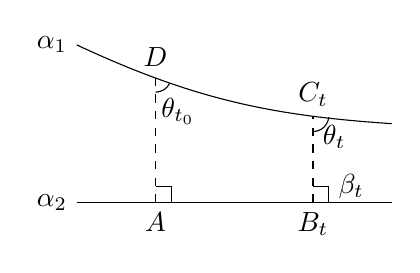
\begin{tikzpicture}
    %\draw[help lines] (-2,0) grid (2,3);
    \draw (-2,2)..controls (-0.5,1.3) and (0.5,1.1).. (2,1);
    \draw (-2,0)--(2,0);
    \draw[dashed] (-1,0)--(-1,1.6);
    \draw[dashed] (1,0)--(1,1.1);
    \draw (-1,0.2)--(-0.8,0.2)--(-0.8,0) (1,0.2)--(1.2,0.2)--(1.2,0);
    \draw (1,0.9) arc [radius=0.2,start angle=-90,end angle=-5];
    
    \node[left] at(-2,0) {$\alpha_2$};
    \node[left] at (-2,2) {$\alpha_1$};
    \node[below right] at (1,1.1) {$\theta_t$};
    \node[right] at (1.2,0.2) {$\beta_t$};
    \node[below] at (-1,0) {$A$};
    \node[below] at (1,0) {$B_t$};
    \node[above] at (1,1.1) {$C_t$};
    \node[above] at (-1,1.6) {$D$};
    
    \draw (-1,1.4) arc [radius=0.2,start angle=-90,end angle=-25];
    \node[below right] at (-1.05,1.45) {$\theta_{t_0}$};
    \end{tikzpicture}
    \caption{Two asymptotic rays and $\theta_t$}
    \label{varying}
\end{figure}

Now assume that $\theta_t\le\frac{\pi}{2}$ for all $t$. Fix one $\beta_{t_0}$ and take a $\beta_t$ for some $t>t_0$. $\beta_{t_0},\beta_t,\alpha_1,\alpha_2$ enclose a quadrilateral $AB_tC_tD$. Glue it with another identical quadrilateral along vertices and edges, we get a flat cone surface homeomorphic to a sphere. The cone points of this sphere consist of the original cone points inside the polygon, cone points in the edges and the vertices $A,B_t,C_t,D$.

Suppose there are only finitely many cone points in both $\alpha_1$ and $\alpha_2$. Then we can always replace $\alpha_i$ by shorter subrays and assume there is no cone point in both rays. Denote the cone points inside the polygon $AB_tC_tD$ by $p_1,\ldots,p_{N_t}$. Each cone point $p_i$ contributes a concentrated curvature $\kappa_i=2\pi-\theta(p_i)<0$, $\kappa_A=\kappa_{B_t}=\pi, \kappa_{C_t}=2\pi-2\theta_t, \kappa_{D}=2\theta_{t_0}$. Apply Gauss-Bonnet theorem, we get
\[\theta_t=\theta_{t_0}+\sum_{i=1}^{N_t}\kappa_i\]

Thus $\theta_t$ is a nondecreasing step function with respect to $t$. Since $\theta_t$ is bounded above by $\frac{\pi}{2}$, $\theta_t$ converges as $t$ goes to infinity and therefore, $\kappa_i$ converges to $0$. Note that these cone points in the polygon come from the lift of finitely many cone points in the surface $S$, so $\kappa_i$ could only take finitely many values, which forces $\kappa_i=0$ for almost all $i$. Therefore, up to taking subrays, $\alpha_1$ and $\alpha_2$ bound a flat region, and it must be a flat half strip. In particular, $\theta_t=\frac{\pi}{2}$ for all large enough $t$. 

The remaining case is that there are infinitely many cone points in at least one of the geodesic rays $\alpha_1,\alpha_2$. For a cone point $p$ in the edges of the polygon, it could contribute a curvature arbitrarily close to 0, which makes it possible that $\theta_t$ converges to $\frac{\pi}{2}$ and $\theta_t\ne \frac{\pi}{2}$.
\end{proof}

\end{document}
